\documentclass[utf8x]{beamer}

\mode<presentation>
{
  \usetheme{Warsaw}

  %\setbeamercovered{transparent}
}

\usepackage[english]{babel}

\usepackage[utf8x]{inputenc}

\usepackage{times}
\usepackage[T1]{fontenc}
\usepackage{color}

\title{The speed of PyPy}

\author{Maciej Fijałkowski}

\institute[merlinux GmbH]
{ merlinux GmbH }

\date{RuPy, November 7th 2009, Poznań}

\begin{document}

\begin{frame}
  \titlepage
\end{frame}

\begin{frame}

  \frametitle{Story about Python's speed}
  \begin{figure}
    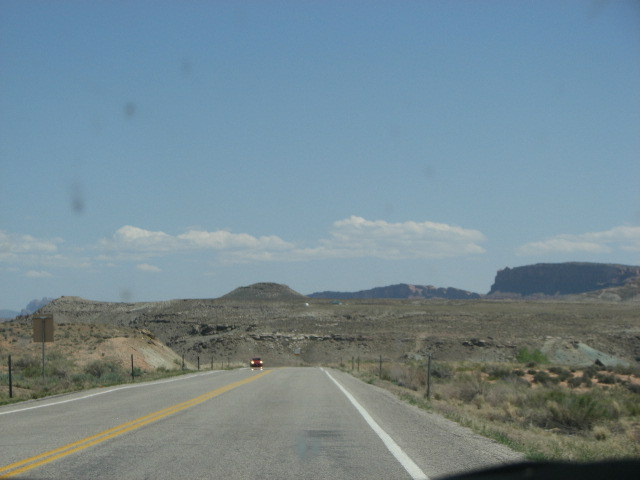
\includegraphics[width=.8\textwidth]{img1.jpg}
  \end{figure}

\end{frame}

\begin{frame}
  \frametitle{Speed of Python}
  \begin{itemize}
     \item Python is slow
  \end{itemize}
  \pause
  \begin{figure}
    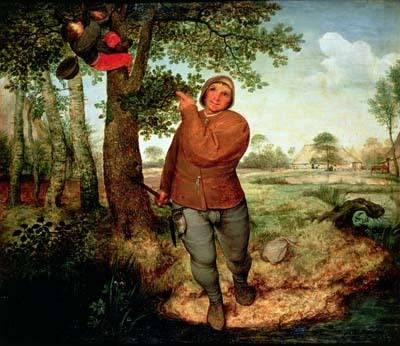
\includegraphics[width=.6\textwidth]{peasant_and_birdnester-400.jpg}
  \end{figure}
  
\end{frame}

\begin{frame}
  \frametitle{Speed of Python}
  \begin{itemize}
    \item Is Python really slow?
      \pause
    \item Sometimes, for some usecases
      \pause
    \item Let's have a look at some examples
  \end{itemize}

\end{frame}

\begin{frame}
  \frametitle{Nomenclature}
  \begin{itemize}
    \item Python - a programming language
    \item CPython - main implementation of Python
    \item JVM - Java Virtual Machine - VM used to run Java, among others
    \item JIT - Just in time compiler
    \item Psyco - JIT for Python
  \end{itemize}
\end{frame}

\begin{frame}
  \frametitle{Example run}
  \begin{itemize}
    \item Float example, stolen from factor blog
  \end{itemize}
  \vspace{.5cm}
  \begin{tabular}{| l | c | r |}
    \hline
    & CPython & Java (hotspot client mode) \\
    Average of 10 runs: & 7.6s & 0.77s \\
    \hline
  \end{tabular}
  \vspace{.5cm}
  \pause
  \begin{itemize}
    \item Python is 10x slower than Java
      \pause
    \item Python is 10x slower than Java on this particular benchmark
      \pause
    \item CPython is 10x slower than Java on this particular benchmark
  \end{itemize}
\end{frame}

\begin{frame}
  \frametitle{More about this example}
  \begin{tabular}{| l | c | c | c | c |}
    \hline
    & CPython & JVM & Psyco & PyPy \\
    Average of 10 runs & 7.6s & 0.77s & 4.4s & 1.3s \\
    \hline
  \end{tabular}
  \vspace{.5cm}
  \pause
  \begin{itemize}
    \item So, it's CPython that is slow on this particular benchmark
      \pause
    \item Same example, using numpy and vectorization about 3x faster than JVM
  \end{itemize}
\end{frame}

\begin{frame}
  \frametitle{Python's speed}
  \begin{itemize}
    \item Instead of: ``Why is Python slow?''
      \pause
    \item Better: ``Why is Python hard to optimize?''
      \pause
    \item Even better: ``How are we going to fix it?''
  \end{itemize}
\end{frame}

\begin{frame}
  \frametitle{Some evidence}
  \begin{figure}
    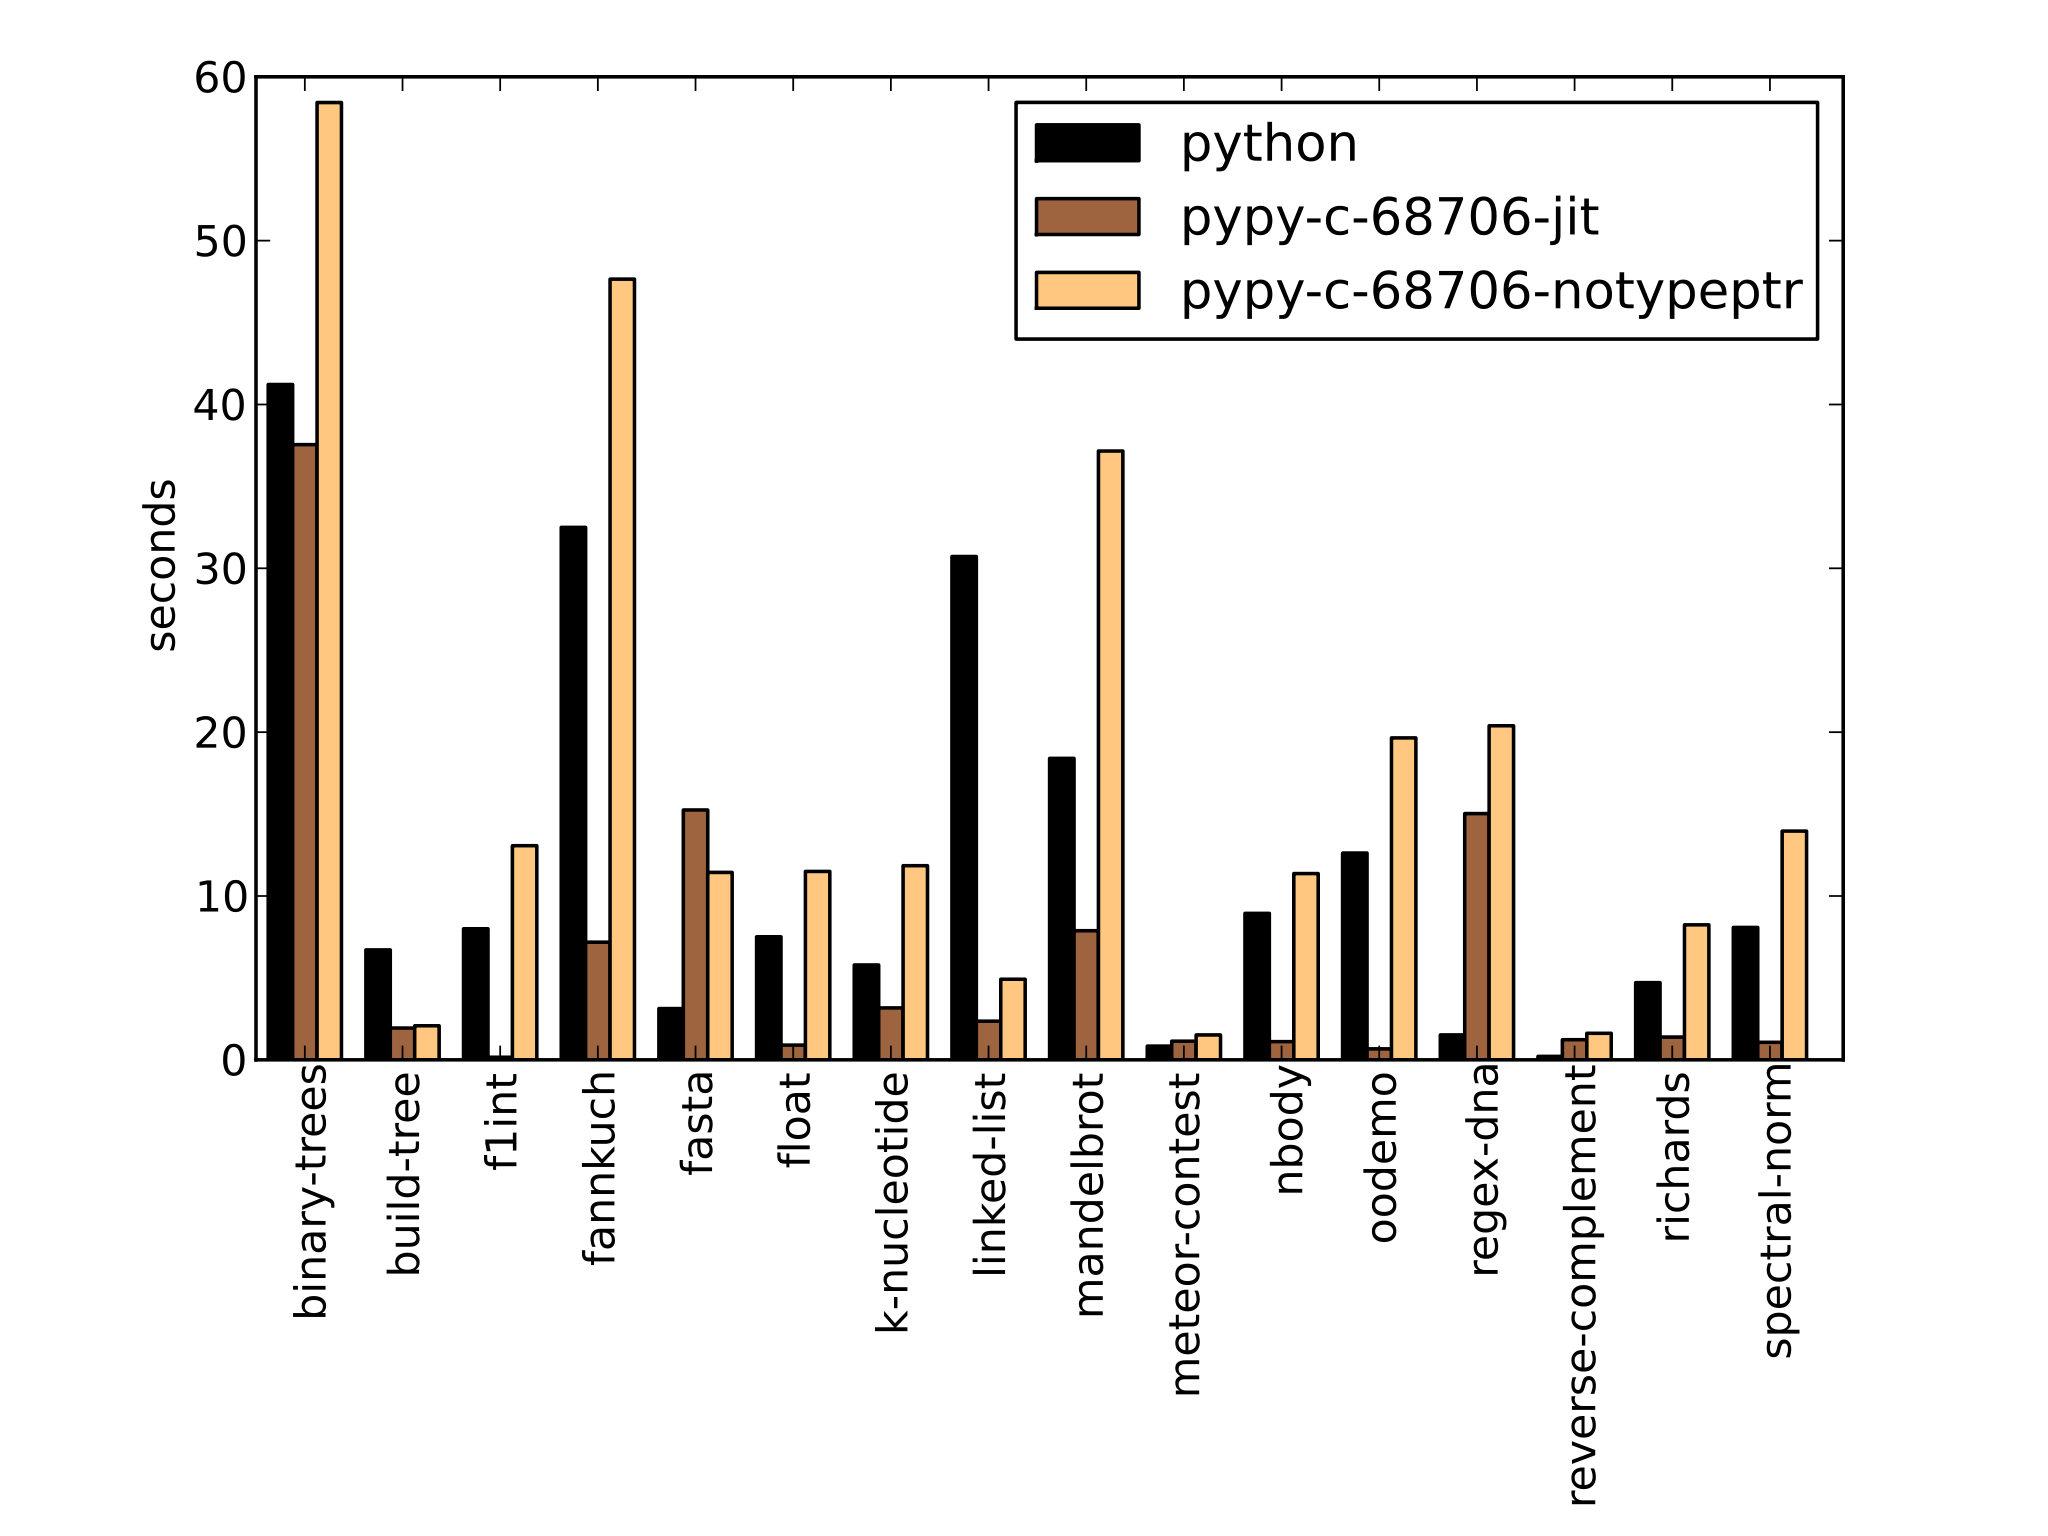
\includegraphics[width=1.0\textwidth]{time.png}
  \end{figure}
\end{frame}

\begin{frame}
  \frametitle{Why is Python hard to optimize?}
  \begin{itemize}
    \item Duck typing (dynamic dispatch)
    \item Frames
    \item Object encapsulation
    \item Dictionaries of instances
    \item Changing globals
    \item Ability to dynamically change builtins
  \end{itemize}
\end{frame}

\begin{frame}
  \frametitle{Duck typing}
  \begin{itemize}
    \item Dispatching over item type
    \item {\tt z = x + y}
    \item Needs to check what the type of {\tt x} and {\tt y} is
  \end{itemize}
\end{frame}

\begin{frame}
  \frametitle{Frames}
  \begin{itemize}
    \item Python interpreters use frames on heap (instead of stack)
    \item Locals are stored on those frames
    \item Intermediate results are store on valuestack of frames
    \item In fact, you can access frames via {\tt sys.\_getframe() or
      traceback}
  \end{itemize}
\end{frame}

\begin{frame}
  \frametitle{Object encapsulation}
  \begin{itemize}
    \item Also called boxing
    \item Each object, even {\tt int}, has to be boxed
    \item Requires allocations and indirection
  \end{itemize}
\end{frame}

\begin{frame}
  \frametitle{Example - addition}
  \begin{itemize}
    \item {\tt z = x + y}
    \item read value for {\tt x} from frame, store on valuestack
    \item read value for {\tt x} from frame, store on valuestack
    \item allocate new integer
    \item read two values from valuestack, add and store the result in
      freshly allocated integer
    \item move the result from valuestack to locals
      \pause
    \item {\color{red} in fact, should be one assembler instruction}
  \end{itemize}
\end{frame}

\begin{frame}
  \frametitle{Dictionaries of instances}
  \begin{itemize}
    \item Need to perform a dictionary lookup for {\tt x.y}
    \item There are {\bf three} lookups per method call
      (descriptor, object, type)
    \item {\bf Two} for attribute access
      (descriptor, object)
    \item Looks like list lookup should be enough
  \end{itemize}
\end{frame}

\begin{frame}
  \frametitle{Changing globals}
  \begin{itemize}
    \item Global symbols can change at any moment in time
    \item Makes inlining hard
    \item Requires global dict lookups, even for constants
  \end{itemize}
\end{frame}

\begin{frame}
  \frametitle{Ability to dynamically change builtins}
  \begin{itemize}
    \item You can say {\tt int = my\_function}
    \item But you can't {\tt int.\_\_add\_\_ = my\_method}
    \item Still messes up optimizations
    \item Global lookup is also a dictionary lookup, even if globals
      don't change
  \end{itemize}
\end{frame}

\begin{frame}
  \frametitle{Interpreting vs compiling}
  \begin{itemize}
    \item Apparently, processors are good at branch prediction
    \item We didn't measure much of a difference, less than 2x overall
  \end{itemize}
\end{frame}

\begin{frame}
  \frametitle{CPython specific problems}
  \begin{itemize}
    \item In general, CPython is fairly well optimized
    \item refcounting is an inefficient garbage collection scheme
    \item GIL
  \end{itemize}
\end{frame}

\begin{frame}
  \frametitle{Dynamic compilation to the rescue}
  \begin{itemize}
    \item You don't pay for feature, until you actually use it
    \item In static compilation, compiler has to prove that bad
      things can't happen
    \item Impossible in Python
    \item With dynamic compilation, you just throw away compiled
      code in case things go wrong or start over
  \end{itemize}
\end{frame}

\begin{frame}
  \frametitle{Dealing with frames}
  \begin{itemize}
    \item Allocate frame
      \pause
    \item Use C stack, but remember where frame fields are
      living on the stack
      \pause
    \item Be able to reconstruct frame on demand (for example
      {\tt sys.\_getframe() was called})
      \pause
    \item The effect is that you don't pay for frames, unless
      you really use them
  \end{itemize}
\end{frame}

\begin{frame}
  \frametitle{Dealing with dynamic dispatch}
  \begin{itemize}
    \item The answer is to simply specialize over types
    \item Provides possibly multiple versions of compiled code for
      single Python code
  \end{itemize}
\end{frame}

\begin{frame}
  \frametitle{Dealing with object encapsulation}
  \begin{itemize}
    \item ``Virtual objects''
    \item Also known as escape analysis
    \item If object does not ``escape'', don't allocate it at all
  \end{itemize}
\end{frame}

\begin{frame}
  \frametitle{How does it work in practice?}
  \begin{itemize}
    \pause
    \item Pretty well
      \pause
    \item A reasonable speedup over CPython
  \end{itemize}
\end{frame}

\begin{frame}
  \frametitle{Dealing with attribute access}
  \begin{itemize}
    \item Fairly complex task
    \item Sharing dict, more or less the same effect as V8's hidden
      classes
      \pause
    \item Python is a very complex language
    \item Shadowing methods with attributes
    \item Descriptors before attributes
  \end{itemize}
\end{frame}

\begin{frame}
  \frametitle{Other important optimizations}
  \begin{itemize}
    \item Caching globals
    \item Caching builtins
    \item A lot of smaller ones
  \end{itemize}
\end{frame}

\begin{frame}
  \frametitle{Bird's view of JIT}
  \begin{itemize}
    \item Mixed mode - interpreter \& JIT for hot paths
    \item Tracing JIT (like TraceMonkey), not up-front
    \item 
  \end{itemize}
\end{frame}

\begin{frame}
  \frametitle{CPython vs PyPy}
  \begin{itemize}
    \item I use CPython for everyday usage
      \pause
    \item But personally, I hope to change it in next months
      \pause
    \item ... in places where performance matters, but that don't
      depend on third party C modules (like numpy)
      \pause
    \item ... like building and developing PyPy
  \end{itemize}
\end{frame}

\begin{frame}
  \frametitle{Status of PyPy}
  \begin{itemize}
    \item Very compliant Python interpreter
    \item Most of important stdlib modules
    \item Differencies are agreed to be implementation details
      \pause
    \item {\color{red} or bugs}
  \end{itemize}
\end{frame}

\begin{frame}
  \frametitle{Examples of working programs}
  \begin{itemize}
    \item Django (sqlite only)
    \item Twisted
    \item PyPy's translation toolchain
    \item ctypes
  \end{itemize}
\end{frame}

\begin{frame}
  \frametitle{Status of JIT}
  \begin{itemize}
    \item Because the way it's constructed, handles all Python language
      features (unlike for example {\bf Psyco})
    \item Changes very quickly these days
    \item Ready for cautious tests
    \item Not ready as a drop-in replacement of CPython
      \pause
    \item {\color{green} yet!}
  \end{itemize}
\end{frame}

\begin{frame}
  \frametitle{Adapt today!}
  \begin{itemize}
    \item A fact: People rely on deep obscure features of language
    \item Examples:
      \pause
      \begin{itemize}
        \item {\tt except ImportError, e: \\ \quad if str(e) != ...:
          raise}
          \pause
        \item Exact naming of list comprehension variable
          \pause
        \item Reliance on reference counting
      \end{itemize}
  \end{itemize}
\end{frame}

\begin{frame}
  \frametitle{Profit tomorrow!}
  \begin{itemize}
    \item We plan to release JIT-ready version somewhere early 2010
      \pause
    \item It should be able to speed up real-world programs
  \end{itemize}
\end{frame}

\begin{frame}
  \frametitle{How you can help}
  \begin{itemize}
    \item It's all open source after all ...
    \item Try running existing programs
    \item Profile, report bugs
      \pause
    \item Talk to your boss
  \end{itemize}
\end{frame}

\begin{frame}
  \frametitle{Thank you!}
  \begin{itemize}
    \item This talk is already online (with all examples):
      {\tt http://codespeak.net/svn/pypy/dist/extradoc/talk/rupy2009/talk.pdf}
    \item {\tt http://morepypy.blogspot.com}
    \item \#pypy on freenode
    \item If you want to know more about PyPy, feel free to bug me
      around (like, how does the JIT work?)
    \item Any questions?
  \end{itemize}
\end{frame}

\end{document}

